\documentclass{article}
\usepackage[utf8]{inputenc}
\usepackage{cite}
\usepackage{amsmath,amssymb,amsfonts}
\usepackage{algorithmic}
\usepackage{graphicx}
\usepackage{textcomp}
\usepackage{xcolor}
\usepackage{braket}
\usepackage{biblatex}
\usepackage{float}
\usepackage{hyperref}

\title{Mesures et courbes}
\author{Antoine Mingasson}
\date{April 2021}

\begin{document}

\maketitle

\section{Introduction}

Ce document présente quelques mesures effectuées dans le cadre de mon stage.
Les mesures représentes des valeurs relevées depuis un analyseur de réseau, le PICOVNA.\\
\\
Les valeurs présentées dans ce document représente l'atténuation de la puissance transmise dans différents milieux. J'ai effectué des mesures dans l'air, l'eau douce et l'eau salée, à plusieurs distances et plusieurs fréquences.\\
\\
Les antennes utilisées pour la transmission sont nommées "antenne fouet", "antenne large bande" et "antenne LoRa". Les deux premières sont des antennes du commerce, la 3ieme est une antenne LoRa sans datasheet.\\

Lien antennes :

\section{Mesures}
Il est important de noter que les mesures faites avec l'analyseur de réseau sont sujettes à quelques variations, j'ai essayé de minimiser ce phénomène de variation en utilisant "l'averaging" présent sur l'analyseur et en effectuant plusieurs mesures en changeant légèrement la configuration ( position et agencement de câbles notamment). L'antenne en céramique semble présenter des variations bien moins fortes cependant.
\\
L'analyseur de réseau utilisé semble montrer que le bruit ambiant apparaît au alentours de -70dB, c'est pourquoi sur le dernier graphes les mesures à plus de 600MHz environ sont noyées dans le bruit. Cependant les mesures en dessous de la barre des 600MHz sont porteuses d'informations.
\\
Utilisation du Filtre FI ??
\section{Graphes antennes}
Les graphes suivants montre la perte de puissance entre l'émetteur et le récepteur.\\

\begin{figure}[H]
    \caption{Absorption en fonction de la fréquence avec l'antenne fouet}
    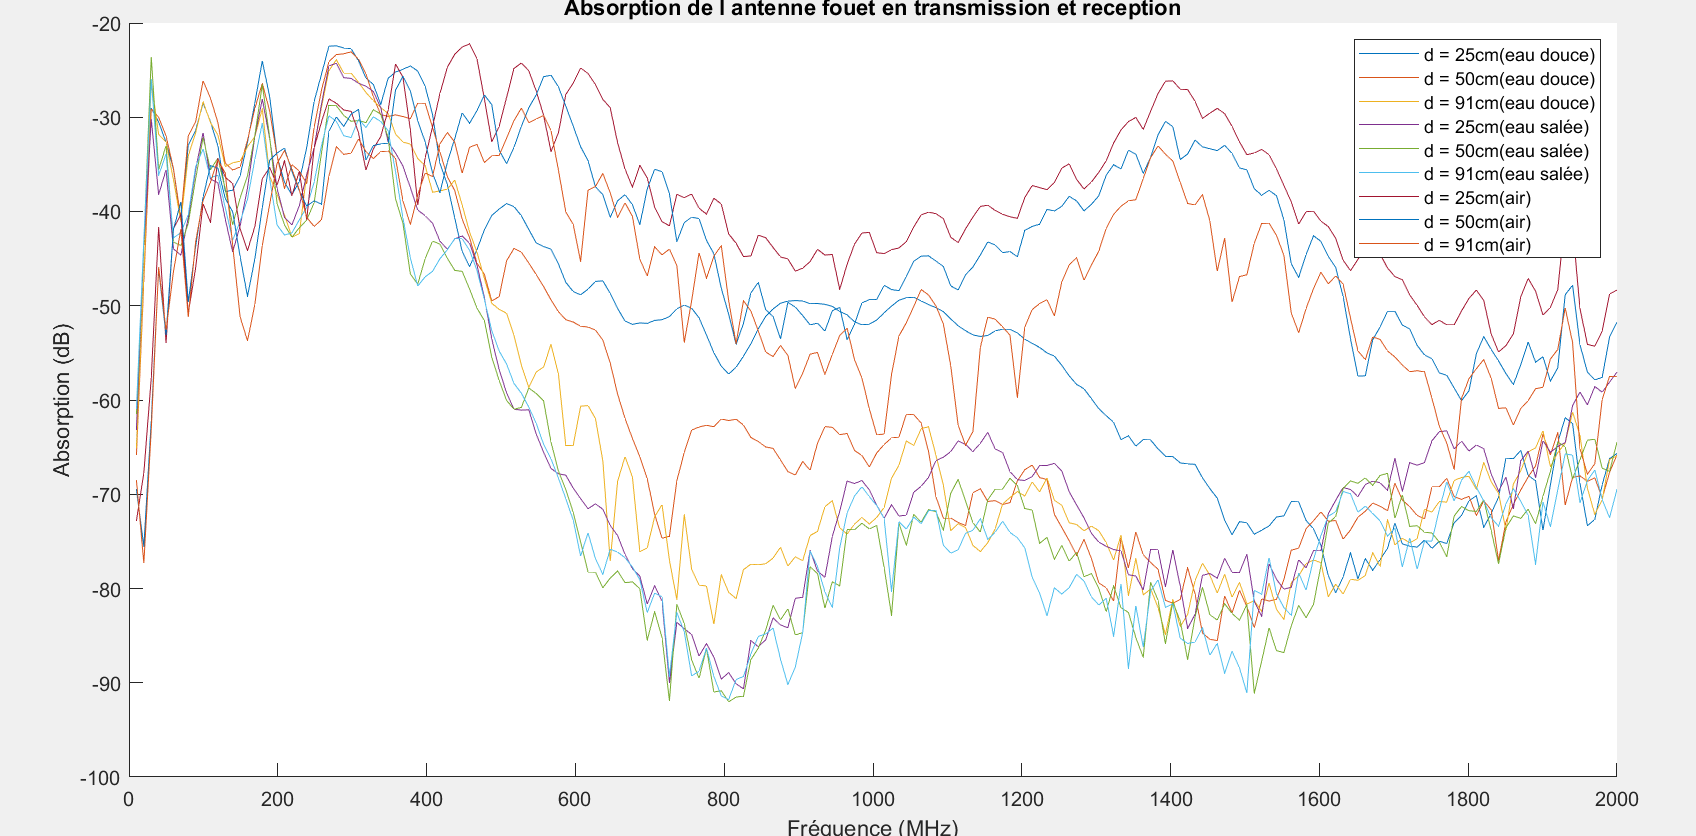
\includegraphics[scale=0.4]{images/abs_fouet.PNG}
    \centering
\end{figure}

\begin{figure}[H]
    \caption{Absorption en fonction de la fréquence avec l'antenne large bande}
    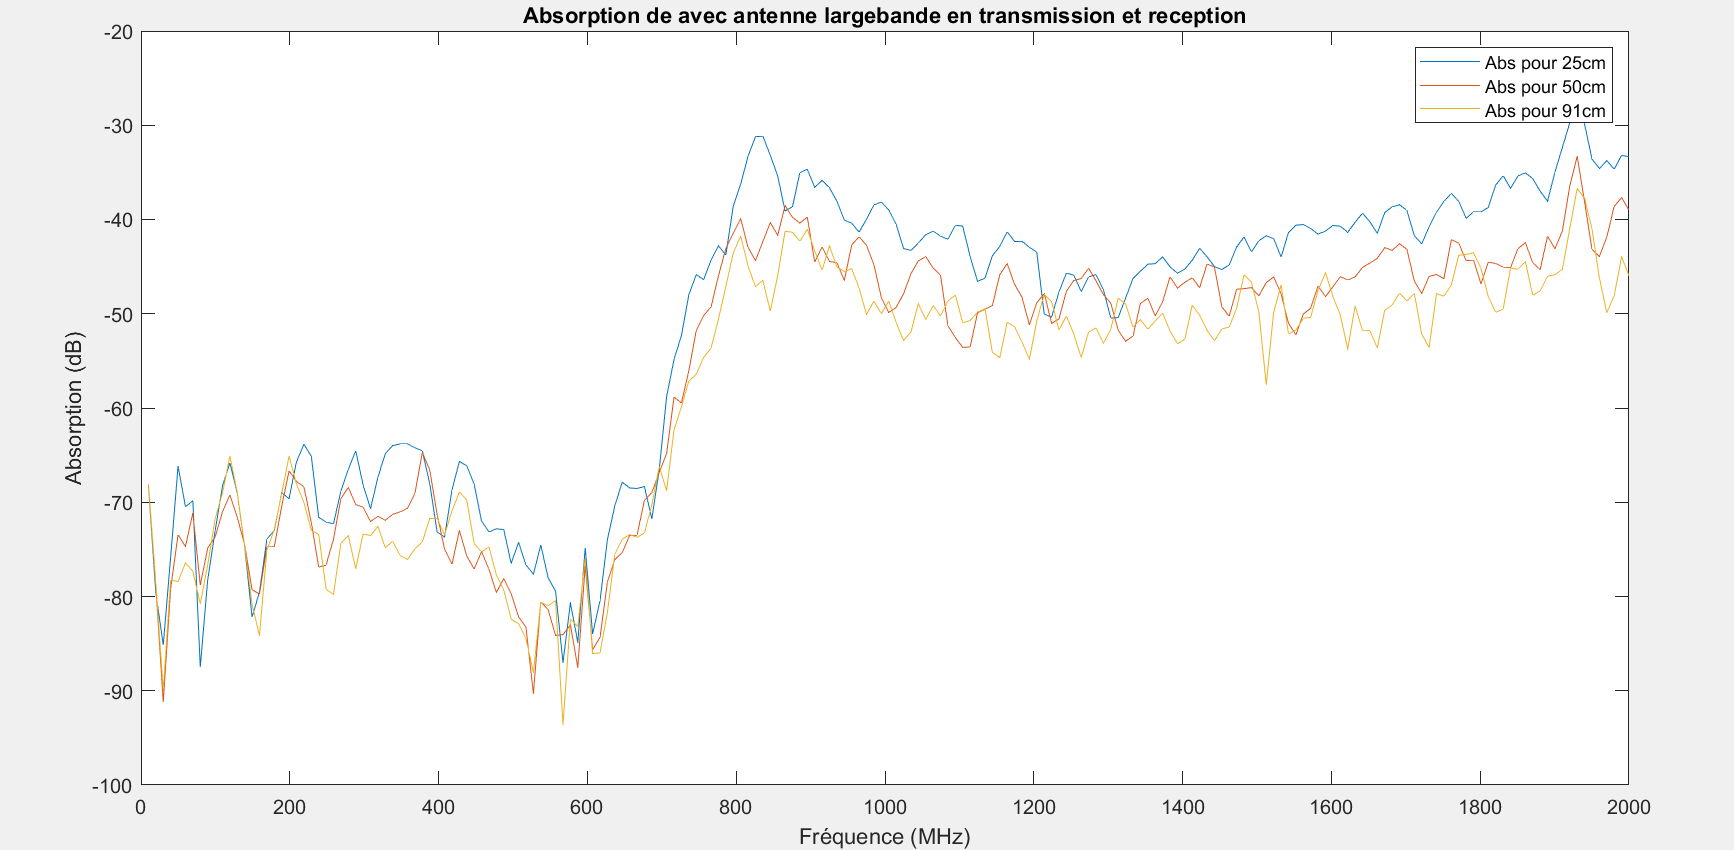
\includegraphics[scale=0.4]{images/abs_large.PNG}
    \centering
\end{figure}

\begin{figure}[H]
    \caption{Absorption en fonction de la fréquence avec l'antenne LoRa}
    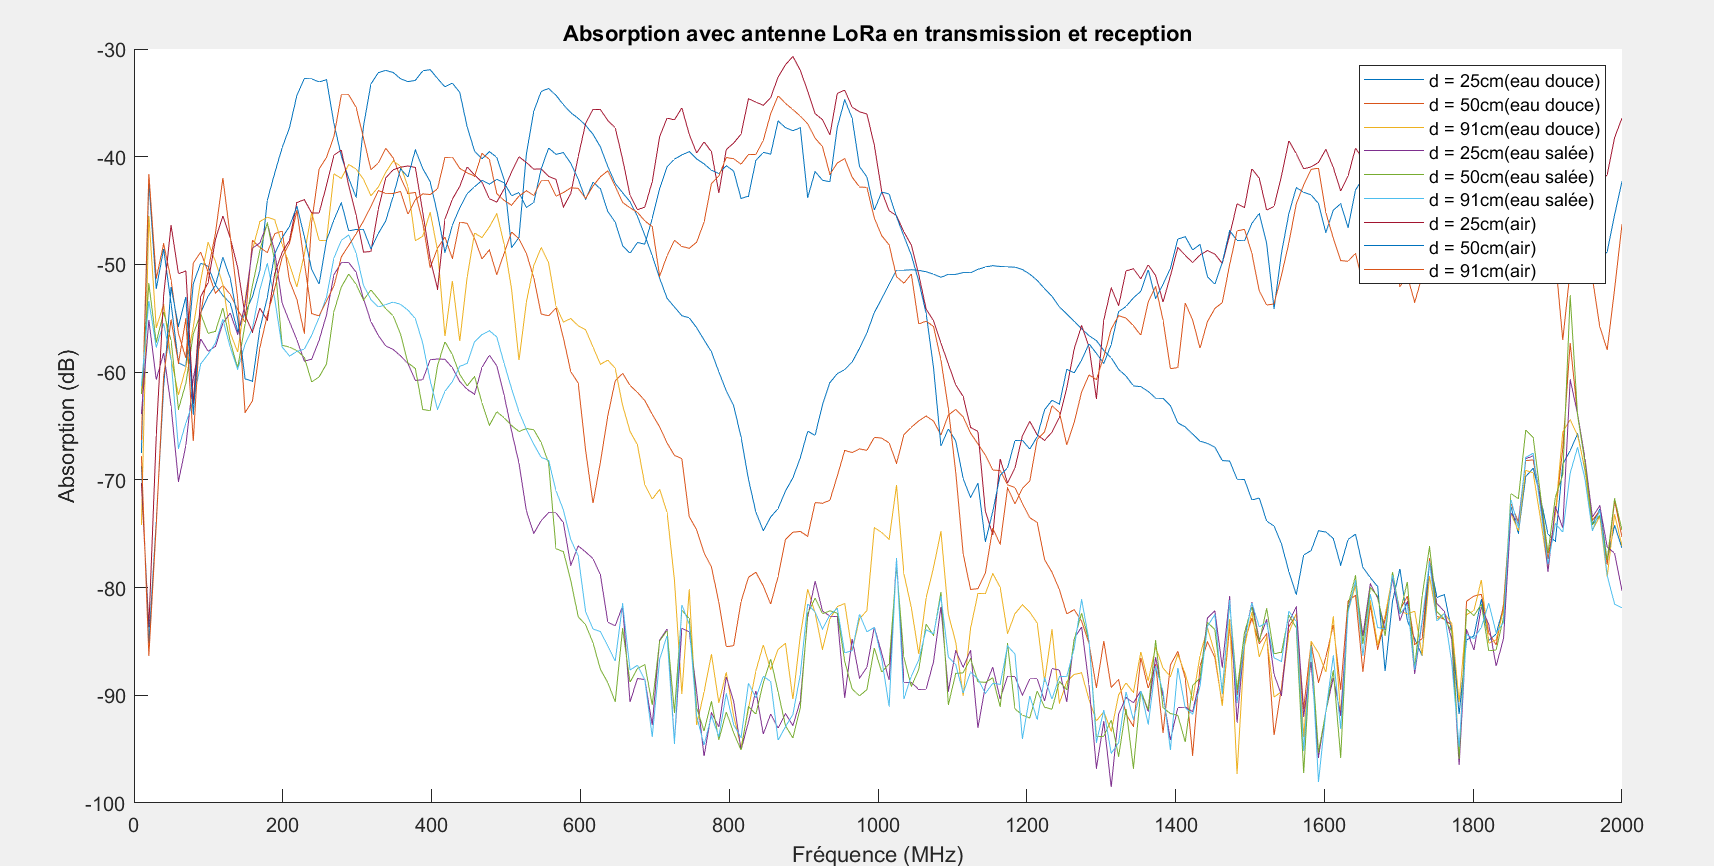
\includegraphics[scale=0.4]{images/abs_lora.PNG}
    \centering
\end{figure}


L'antenne large bande possède une émission à basse fréquence très mauvaise, les relevés dans l'eau salée était uniquement dans le bruit c'est pourquoi je n'ai pas de résultats pour cette antenne.

\section{Analyse et Comparaison à la simulation}

Le graphe suivant représente l'absorption de l'antenne fouet et l'antenne LoRa côte à côte.
On peux remarquer la différence de performance de deux antennes à basses fréquence. Vers 500MHz l'absorption monte en flèche et arrive vite aux limites de l'analyseur de réseau.
On peux aussi remarquer que la distance (25cm,50cm,91cm) entre les antennes lors des mesures ne semble pas impacter les valeurs d'absorption

\begin{figure}[H]
    \caption{Absorption en fonction de la fréquence avec l'antenne fouet et l'antenne LoRa}
    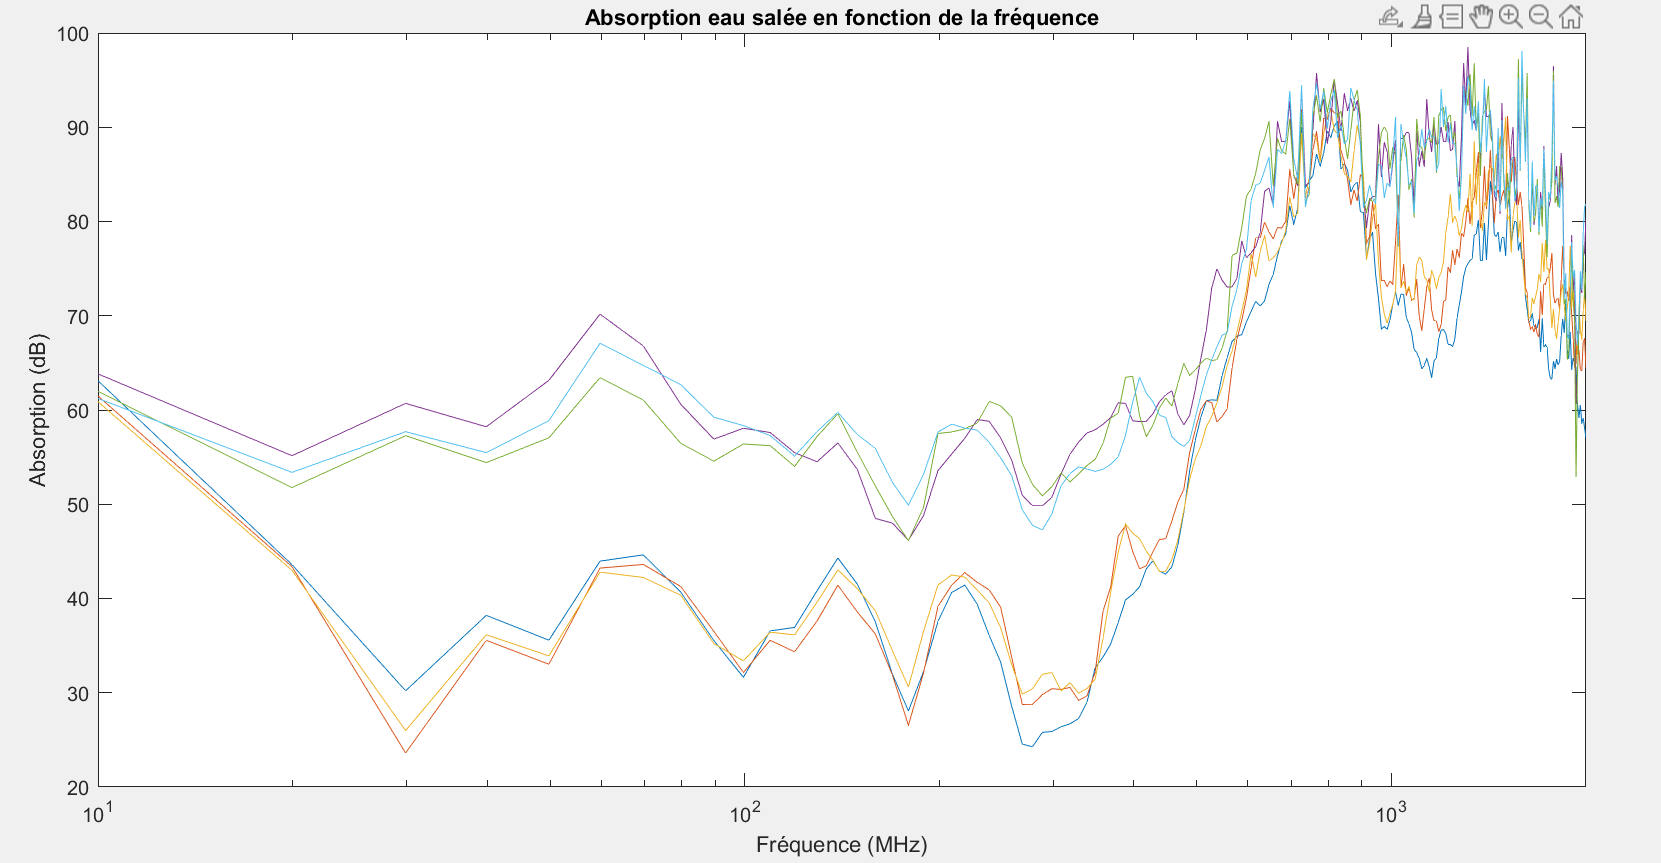
\includegraphics[scale=0.4]{images/abs_lora_fouet.PNG}
    \centering
\end{figure}


Le graphe suivant présente mes résultats par rapport aux simulations

\begin{figure}[H]
    \caption{Absorption en fonction de la fréquence avec l'antenne fouet et l'antenne LoRa comparé aux simulations}
    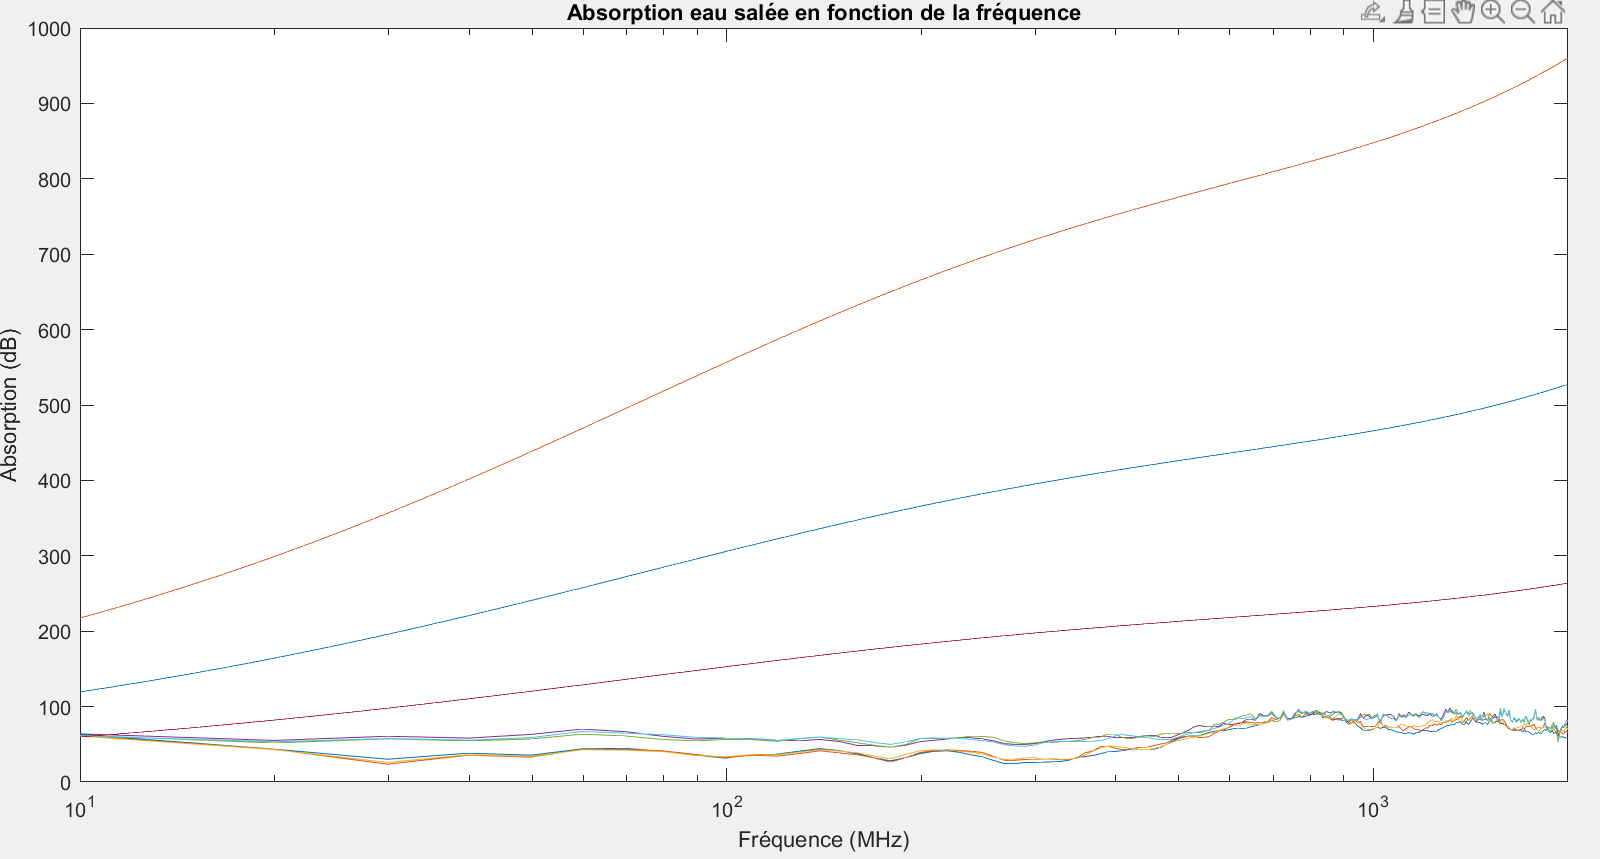
\includegraphics[scale=0.4]{images/comp_avec_simu.PNG}
    \centering
\end{figure}


\section{Observations}

Les résultats observés sont à prendre avec des pincettes car ils ne sont que difficilement comparables avec la théorie(simulation), en effet le bassin à des dimensions faibles et est sujet à des phénomènes perturbateurs(longueur = 98cm, largeur = 38cm, hauteur de l'eau = 34.5cm). On a dans le bassin 128 litres d'eau. Pour simuler l'effet de l'eau salée, j'ai voulu reproduire le milieu marin et j'ai donc incorporé 4.48kg de sel. Une fois le sel dissous, l'eau possédait une conductivité de 4.9 s/m.
Pour le moment je ne sais pas ou se trouve le vrai niveau d'absorption. Les mesures semblent être un peu trop utopiques d'autant plus que les valeurs d'absorptions ne semblent pas changer avec la distance. D'un autre coté la simulation présente des valeurs d'absorption extrêmement élevées.\\
Les solutions possibles pour réussir à comparer la simulation et la pratique serait 



\end{document}
